% Created by tikzDevice version 0.12.3.2 on 2022-02-18 20:50:34
% !TEX encoding = UTF-8 Unicode
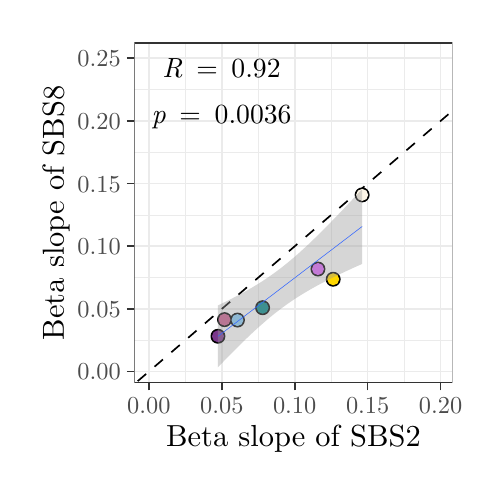
\begin{tikzpicture}[x=1pt,y=1pt]
\definecolor{fillColor}{RGB}{255,255,255}
\path[use as bounding box,fill=fillColor,fill opacity=0.00] (0,0) rectangle (158.99,158.99);
\begin{scope}
\path[clip] (  0.00,  0.00) rectangle (158.99,158.99);
\definecolor{drawColor}{RGB}{255,255,255}
\definecolor{fillColor}{RGB}{255,255,255}

\path[draw=drawColor,line width= 0.6pt,line join=round,line cap=round,fill=fillColor] (  0.00,  0.00) rectangle (158.99,158.99);
\end{scope}
\begin{scope}
\path[clip] ( 38.56, 30.69) rectangle (153.49,153.49);
\definecolor{fillColor}{RGB}{255,255,255}

\path[fill=fillColor] ( 38.56, 30.69) rectangle (153.49,153.49);
\definecolor{drawColor}{gray}{0.92}

\path[draw=drawColor,line width= 0.3pt,line join=round] ( 38.56, 46.03) --
	(153.49, 46.03);

\path[draw=drawColor,line width= 0.3pt,line join=round] ( 38.56, 68.67) --
	(153.49, 68.67);

\path[draw=drawColor,line width= 0.3pt,line join=round] ( 38.56, 91.31) --
	(153.49, 91.31);

\path[draw=drawColor,line width= 0.3pt,line join=round] ( 38.56,113.95) --
	(153.49,113.95);

\path[draw=drawColor,line width= 0.3pt,line join=round] ( 38.56,136.59) --
	(153.49,136.59);

\path[draw=drawColor,line width= 0.3pt,line join=round] ( 56.96, 30.69) --
	( 56.96,153.49);

\path[draw=drawColor,line width= 0.3pt,line join=round] ( 83.32, 30.69) --
	( 83.32,153.49);

\path[draw=drawColor,line width= 0.3pt,line join=round] (109.67, 30.69) --
	(109.67,153.49);

\path[draw=drawColor,line width= 0.3pt,line join=round] (136.03, 30.69) --
	(136.03,153.49);

\path[draw=drawColor,line width= 0.6pt,line join=round] ( 38.56, 34.71) --
	(153.49, 34.71);

\path[draw=drawColor,line width= 0.6pt,line join=round] ( 38.56, 57.35) --
	(153.49, 57.35);

\path[draw=drawColor,line width= 0.6pt,line join=round] ( 38.56, 79.99) --
	(153.49, 79.99);

\path[draw=drawColor,line width= 0.6pt,line join=round] ( 38.56,102.63) --
	(153.49,102.63);

\path[draw=drawColor,line width= 0.6pt,line join=round] ( 38.56,125.27) --
	(153.49,125.27);

\path[draw=drawColor,line width= 0.6pt,line join=round] ( 38.56,147.91) --
	(153.49,147.91);

\path[draw=drawColor,line width= 0.6pt,line join=round] ( 43.78, 30.69) --
	( 43.78,153.49);

\path[draw=drawColor,line width= 0.6pt,line join=round] ( 70.14, 30.69) --
	( 70.14,153.49);

\path[draw=drawColor,line width= 0.6pt,line join=round] ( 96.49, 30.69) --
	( 96.49,153.49);

\path[draw=drawColor,line width= 0.6pt,line join=round] (122.85, 30.69) --
	(122.85,153.49);

\path[draw=drawColor,line width= 0.6pt,line join=round] (149.21, 30.69) --
	(149.21,153.49);
\definecolor{drawColor}{RGB}{0,0,0}

\path[draw=drawColor,line width= 0.6pt,dash pattern=on 4pt off 4pt ,line join=round] (  3.37,  0.00) -- (158.99,133.68);
\definecolor{fillColor}{RGB}{0,0,0}

\path[draw=drawColor,line width= 0.4pt,line join=round,line cap=round,fill=fillColor] (110.40, 68.09) circle (  2.50);

\path[draw=drawColor,line width= 0.4pt,line join=round,line cap=round,fill=fillColor] ( 71.13, 53.49) circle (  2.50);

\path[draw=drawColor,line width= 0.4pt,line join=round,line cap=round,fill=fillColor] (120.86, 98.56) circle (  2.50);

\path[draw=drawColor,line width= 0.4pt,line join=round,line cap=round,fill=fillColor] ( 84.89, 57.80) circle (  2.50);

\path[draw=drawColor,line width= 0.4pt,line join=round,line cap=round,fill=fillColor] ( 68.76, 47.48) circle (  2.50);

\path[draw=drawColor,line width= 0.4pt,line join=round,line cap=round,fill=fillColor] (104.89, 71.77) circle (  2.50);

\path[draw=drawColor,line width= 0.4pt,line join=round,line cap=round,fill=fillColor] ( 75.80, 53.34) circle (  2.50);
\definecolor{drawColor}{RGB}{255,215,0}
\definecolor{fillColor}{RGB}{255,215,0}

\path[draw=drawColor,line width= 0.4pt,line join=round,line cap=round,fill=fillColor] (110.40, 68.09) circle (  1.96);
\definecolor{drawColor}{RGB}{205,96,144}
\definecolor{fillColor}{RGB}{205,96,144}

\path[draw=drawColor,line width= 0.4pt,line join=round,line cap=round,fill=fillColor] ( 71.13, 53.49) circle (  1.96);
\definecolor{drawColor}{RGB}{253,245,230}
\definecolor{fillColor}{RGB}{253,245,230}

\path[draw=drawColor,line width= 0.4pt,line join=round,line cap=round,fill=fillColor] (120.86, 98.56) circle (  1.96);
\definecolor{drawColor}{RGB}{0,139,139}
\definecolor{fillColor}{RGB}{0,139,139}

\path[draw=drawColor,line width= 0.4pt,line join=round,line cap=round,fill=fillColor] ( 84.89, 57.80) circle (  1.96);
\definecolor{drawColor}{RGB}{122,55,139}
\definecolor{fillColor}{RGB}{122,55,139}

\path[draw=drawColor,line width= 0.4pt,line join=round,line cap=round,fill=fillColor] ( 68.76, 47.48) circle (  1.96);
\definecolor{drawColor}{RGB}{224,102,255}
\definecolor{fillColor}{RGB}{224,102,255}

\path[draw=drawColor,line width= 0.4pt,line join=round,line cap=round,fill=fillColor] (104.89, 71.77) circle (  1.96);
\definecolor{drawColor}{RGB}{135,206,250}
\definecolor{fillColor}{RGB}{135,206,250}

\path[draw=drawColor,line width= 0.4pt,line join=round,line cap=round,fill=fillColor] ( 75.80, 53.34) circle (  1.96);
\definecolor{fillColor}{RGB}{153,153,153}

\path[fill=fillColor,fill opacity=0.40] ( 68.76, 58.62) --
	( 69.42, 58.94) --
	( 70.08, 59.26) --
	( 70.73, 59.58) --
	( 71.39, 59.90) --
	( 72.05, 60.23) --
	( 72.71, 60.55) --
	( 73.37, 60.89) --
	( 74.03, 61.22) --
	( 74.69, 61.56) --
	( 75.35, 61.91) --
	( 76.01, 62.25) --
	( 76.67, 62.60) --
	( 77.33, 62.96) --
	( 77.99, 63.32) --
	( 78.65, 63.69) --
	( 79.31, 64.06) --
	( 79.97, 64.43) --
	( 80.63, 64.81) --
	( 81.29, 65.20) --
	( 81.95, 65.60) --
	( 82.61, 66.00) --
	( 83.27, 66.40) --
	( 83.93, 66.82) --
	( 84.59, 67.24) --
	( 85.25, 67.66) --
	( 85.91, 68.10) --
	( 86.56, 68.54) --
	( 87.22, 68.99) --
	( 87.88, 69.45) --
	( 88.54, 69.92) --
	( 89.20, 70.40) --
	( 89.86, 70.88) --
	( 90.52, 71.37) --
	( 91.18, 71.87) --
	( 91.84, 72.38) --
	( 92.50, 72.90) --
	( 93.16, 73.43) --
	( 93.82, 73.96) --
	( 94.48, 74.51) --
	( 95.14, 75.06) --
	( 95.80, 75.62) --
	( 96.46, 76.18) --
	( 97.12, 76.76) --
	( 97.78, 77.34) --
	( 98.44, 77.93) --
	( 99.10, 78.53) --
	( 99.76, 79.13) --
	(100.42, 79.74) --
	(101.08, 80.35) --
	(101.74, 80.97) --
	(102.39, 81.60) --
	(103.05, 82.23) --
	(103.71, 82.87) --
	(104.37, 83.51) --
	(105.03, 84.16) --
	(105.69, 84.81) --
	(106.35, 85.47) --
	(107.01, 86.13) --
	(107.67, 86.79) --
	(108.33, 87.46) --
	(108.99, 88.13) --
	(109.65, 88.81) --
	(110.31, 89.49) --
	(110.97, 90.17) --
	(111.63, 90.85) --
	(112.29, 91.54) --
	(112.95, 92.23) --
	(113.61, 92.92) --
	(114.27, 93.61) --
	(114.93, 94.31) --
	(115.59, 95.01) --
	(116.25, 95.71) --
	(116.91, 96.41) --
	(117.56, 97.11) --
	(118.22, 97.82) --
	(118.88, 98.53) --
	(119.54, 99.24) --
	(120.20, 99.95) --
	(120.86,100.66) --
	(120.86, 73.63) --
	(120.20, 73.33) --
	(119.54, 73.04) --
	(118.88, 72.74) --
	(118.22, 72.45) --
	(117.56, 72.15) --
	(116.91, 71.85) --
	(116.25, 71.54) --
	(115.59, 71.24) --
	(114.93, 70.93) --
	(114.27, 70.62) --
	(113.61, 70.31) --
	(112.95, 70.00) --
	(112.29, 69.68) --
	(111.63, 69.36) --
	(110.97, 69.04) --
	(110.31, 68.72) --
	(109.65, 68.39) --
	(108.99, 68.06) --
	(108.33, 67.73) --
	(107.67, 67.39) --
	(107.01, 67.05) --
	(106.35, 66.71) --
	(105.69, 66.36) --
	(105.03, 66.00) --
	(104.37, 65.65) --
	(103.71, 65.28) --
	(103.05, 64.92) --
	(102.39, 64.54) --
	(101.74, 64.17) --
	(101.08, 63.78) --
	(100.42, 63.39) --
	( 99.76, 63.00) --
	( 99.10, 62.60) --
	( 98.44, 62.19) --
	( 97.78, 61.77) --
	( 97.12, 61.35) --
	( 96.46, 60.92) --
	( 95.80, 60.48) --
	( 95.14, 60.03) --
	( 94.48, 59.58) --
	( 93.82, 59.12) --
	( 93.16, 58.65) --
	( 92.50, 58.17) --
	( 91.84, 57.68) --
	( 91.18, 57.19) --
	( 90.52, 56.68) --
	( 89.86, 56.17) --
	( 89.20, 55.65) --
	( 88.54, 55.12) --
	( 87.88, 54.58) --
	( 87.22, 54.04) --
	( 86.56, 53.48) --
	( 85.91, 52.92) --
	( 85.25, 52.35) --
	( 84.59, 51.77) --
	( 83.93, 51.19) --
	( 83.27, 50.60) --
	( 82.61, 50.00) --
	( 81.95, 49.40) --
	( 81.29, 48.78) --
	( 80.63, 48.17) --
	( 79.97, 47.54) --
	( 79.31, 46.91) --
	( 78.65, 46.28) --
	( 77.99, 45.64) --
	( 77.33, 45.00) --
	( 76.67, 44.35) --
	( 76.01, 43.69) --
	( 75.35, 43.04) --
	( 74.69, 42.37) --
	( 74.03, 41.71) --
	( 73.37, 41.04) --
	( 72.71, 40.37) --
	( 72.05, 39.69) --
	( 71.39, 39.01) --
	( 70.73, 38.33) --
	( 70.08, 37.65) --
	( 69.42, 36.96) --
	( 68.76, 36.27) --
	cycle;

\path[] ( 68.76, 58.62) --
	( 69.42, 58.94) --
	( 70.08, 59.26) --
	( 70.73, 59.58) --
	( 71.39, 59.90) --
	( 72.05, 60.23) --
	( 72.71, 60.55) --
	( 73.37, 60.89) --
	( 74.03, 61.22) --
	( 74.69, 61.56) --
	( 75.35, 61.91) --
	( 76.01, 62.25) --
	( 76.67, 62.60) --
	( 77.33, 62.96) --
	( 77.99, 63.32) --
	( 78.65, 63.69) --
	( 79.31, 64.06) --
	( 79.97, 64.43) --
	( 80.63, 64.81) --
	( 81.29, 65.20) --
	( 81.95, 65.60) --
	( 82.61, 66.00) --
	( 83.27, 66.40) --
	( 83.93, 66.82) --
	( 84.59, 67.24) --
	( 85.25, 67.66) --
	( 85.91, 68.10) --
	( 86.56, 68.54) --
	( 87.22, 68.99) --
	( 87.88, 69.45) --
	( 88.54, 69.92) --
	( 89.20, 70.40) --
	( 89.86, 70.88) --
	( 90.52, 71.37) --
	( 91.18, 71.87) --
	( 91.84, 72.38) --
	( 92.50, 72.90) --
	( 93.16, 73.43) --
	( 93.82, 73.96) --
	( 94.48, 74.51) --
	( 95.14, 75.06) --
	( 95.80, 75.62) --
	( 96.46, 76.18) --
	( 97.12, 76.76) --
	( 97.78, 77.34) --
	( 98.44, 77.93) --
	( 99.10, 78.53) --
	( 99.76, 79.13) --
	(100.42, 79.74) --
	(101.08, 80.35) --
	(101.74, 80.97) --
	(102.39, 81.60) --
	(103.05, 82.23) --
	(103.71, 82.87) --
	(104.37, 83.51) --
	(105.03, 84.16) --
	(105.69, 84.81) --
	(106.35, 85.47) --
	(107.01, 86.13) --
	(107.67, 86.79) --
	(108.33, 87.46) --
	(108.99, 88.13) --
	(109.65, 88.81) --
	(110.31, 89.49) --
	(110.97, 90.17) --
	(111.63, 90.85) --
	(112.29, 91.54) --
	(112.95, 92.23) --
	(113.61, 92.92) --
	(114.27, 93.61) --
	(114.93, 94.31) --
	(115.59, 95.01) --
	(116.25, 95.71) --
	(116.91, 96.41) --
	(117.56, 97.11) --
	(118.22, 97.82) --
	(118.88, 98.53) --
	(119.54, 99.24) --
	(120.20, 99.95) --
	(120.86,100.66);

\path[] (120.86, 73.63) --
	(120.20, 73.33) --
	(119.54, 73.04) --
	(118.88, 72.74) --
	(118.22, 72.45) --
	(117.56, 72.15) --
	(116.91, 71.85) --
	(116.25, 71.54) --
	(115.59, 71.24) --
	(114.93, 70.93) --
	(114.27, 70.62) --
	(113.61, 70.31) --
	(112.95, 70.00) --
	(112.29, 69.68) --
	(111.63, 69.36) --
	(110.97, 69.04) --
	(110.31, 68.72) --
	(109.65, 68.39) --
	(108.99, 68.06) --
	(108.33, 67.73) --
	(107.67, 67.39) --
	(107.01, 67.05) --
	(106.35, 66.71) --
	(105.69, 66.36) --
	(105.03, 66.00) --
	(104.37, 65.65) --
	(103.71, 65.28) --
	(103.05, 64.92) --
	(102.39, 64.54) --
	(101.74, 64.17) --
	(101.08, 63.78) --
	(100.42, 63.39) --
	( 99.76, 63.00) --
	( 99.10, 62.60) --
	( 98.44, 62.19) --
	( 97.78, 61.77) --
	( 97.12, 61.35) --
	( 96.46, 60.92) --
	( 95.80, 60.48) --
	( 95.14, 60.03) --
	( 94.48, 59.58) --
	( 93.82, 59.12) --
	( 93.16, 58.65) --
	( 92.50, 58.17) --
	( 91.84, 57.68) --
	( 91.18, 57.19) --
	( 90.52, 56.68) --
	( 89.86, 56.17) --
	( 89.20, 55.65) --
	( 88.54, 55.12) --
	( 87.88, 54.58) --
	( 87.22, 54.04) --
	( 86.56, 53.48) --
	( 85.91, 52.92) --
	( 85.25, 52.35) --
	( 84.59, 51.77) --
	( 83.93, 51.19) --
	( 83.27, 50.60) --
	( 82.61, 50.00) --
	( 81.95, 49.40) --
	( 81.29, 48.78) --
	( 80.63, 48.17) --
	( 79.97, 47.54) --
	( 79.31, 46.91) --
	( 78.65, 46.28) --
	( 77.99, 45.64) --
	( 77.33, 45.00) --
	( 76.67, 44.35) --
	( 76.01, 43.69) --
	( 75.35, 43.04) --
	( 74.69, 42.37) --
	( 74.03, 41.71) --
	( 73.37, 41.04) --
	( 72.71, 40.37) --
	( 72.05, 39.69) --
	( 71.39, 39.01) --
	( 70.73, 38.33) --
	( 70.08, 37.65) --
	( 69.42, 36.96) --
	( 68.76, 36.27);
\definecolor{drawColor}{RGB}{51,102,255}

\path[draw=drawColor,line width= 0.2pt,line join=round] ( 68.76, 47.45) --
	( 69.42, 47.95) --
	( 70.08, 48.45) --
	( 70.73, 48.95) --
	( 71.39, 49.46) --
	( 72.05, 49.96) --
	( 72.71, 50.46) --
	( 73.37, 50.96) --
	( 74.03, 51.47) --
	( 74.69, 51.97) --
	( 75.35, 52.47) --
	( 76.01, 52.97) --
	( 76.67, 53.48) --
	( 77.33, 53.98) --
	( 77.99, 54.48) --
	( 78.65, 54.98) --
	( 79.31, 55.49) --
	( 79.97, 55.99) --
	( 80.63, 56.49) --
	( 81.29, 56.99) --
	( 81.95, 57.50) --
	( 82.61, 58.00) --
	( 83.27, 58.50) --
	( 83.93, 59.00) --
	( 84.59, 59.51) --
	( 85.25, 60.01) --
	( 85.91, 60.51) --
	( 86.56, 61.01) --
	( 87.22, 61.52) --
	( 87.88, 62.02) --
	( 88.54, 62.52) --
	( 89.20, 63.02) --
	( 89.86, 63.53) --
	( 90.52, 64.03) --
	( 91.18, 64.53) --
	( 91.84, 65.03) --
	( 92.50, 65.54) --
	( 93.16, 66.04) --
	( 93.82, 66.54) --
	( 94.48, 67.04) --
	( 95.14, 67.55) --
	( 95.80, 68.05) --
	( 96.46, 68.55) --
	( 97.12, 69.05) --
	( 97.78, 69.56) --
	( 98.44, 70.06) --
	( 99.10, 70.56) --
	( 99.76, 71.06) --
	(100.42, 71.57) --
	(101.08, 72.07) --
	(101.74, 72.57) --
	(102.39, 73.07) --
	(103.05, 73.58) --
	(103.71, 74.08) --
	(104.37, 74.58) --
	(105.03, 75.08) --
	(105.69, 75.59) --
	(106.35, 76.09) --
	(107.01, 76.59) --
	(107.67, 77.09) --
	(108.33, 77.60) --
	(108.99, 78.10) --
	(109.65, 78.60) --
	(110.31, 79.10) --
	(110.97, 79.61) --
	(111.63, 80.11) --
	(112.29, 80.61) --
	(112.95, 81.11) --
	(113.61, 81.62) --
	(114.27, 82.12) --
	(114.93, 82.62) --
	(115.59, 83.12) --
	(116.25, 83.63) --
	(116.91, 84.13) --
	(117.56, 84.63) --
	(118.22, 85.13) --
	(118.88, 85.64) --
	(119.54, 86.14) --
	(120.20, 86.64) --
	(120.86, 87.14);
\definecolor{drawColor}{RGB}{0,0,0}

\node[text=drawColor,anchor=base west,inner sep=0pt, outer sep=0pt, scale=  1.00] at ( 48.68,141.05) {\itshape R};

\node[text=drawColor,anchor=base west,inner sep=0pt, outer sep=0pt, scale=  1.00] at ( 55.94,141.05) { };

\node[text=drawColor,anchor=base west,inner sep=0pt, outer sep=0pt, scale=  1.00] at ( 60.92,141.05) {=};

\node[text=drawColor,anchor=base west,inner sep=0pt, outer sep=0pt, scale=  1.00] at ( 68.66,141.05) { };

\node[text=drawColor,anchor=base west,inner sep=0pt, outer sep=0pt, scale=  1.00] at ( 73.64,141.05) {0.92};

\node[text=drawColor,anchor=base west,inner sep=0pt, outer sep=0pt, scale=  1.00] at ( 44.79,124.23) {\itshape p};

\node[text=drawColor,anchor=base west,inner sep=0pt, outer sep=0pt, scale=  1.00] at ( 49.88,124.23) { };

\node[text=drawColor,anchor=base west,inner sep=0pt, outer sep=0pt, scale=  1.00] at ( 54.85,124.23) {=};

\node[text=drawColor,anchor=base west,inner sep=0pt, outer sep=0pt, scale=  1.00] at ( 62.60,124.23) { };

\node[text=drawColor,anchor=base west,inner sep=0pt, outer sep=0pt, scale=  1.00] at ( 67.58,124.23) {0.0036};
\definecolor{drawColor}{gray}{0.20}

\path[draw=drawColor,line width= 0.6pt,line join=round,line cap=round] ( 38.56, 30.69) rectangle (153.49,153.49);
\end{scope}
\begin{scope}
\path[clip] (  0.00,  0.00) rectangle (158.99,158.99);
\definecolor{drawColor}{gray}{0.30}

\node[text=drawColor,anchor=base east,inner sep=0pt, outer sep=0pt, scale=  0.88] at ( 33.61, 31.68) {0.00};

\node[text=drawColor,anchor=base east,inner sep=0pt, outer sep=0pt, scale=  0.88] at ( 33.61, 54.32) {0.05};

\node[text=drawColor,anchor=base east,inner sep=0pt, outer sep=0pt, scale=  0.88] at ( 33.61, 76.96) {0.10};

\node[text=drawColor,anchor=base east,inner sep=0pt, outer sep=0pt, scale=  0.88] at ( 33.61, 99.60) {0.15};

\node[text=drawColor,anchor=base east,inner sep=0pt, outer sep=0pt, scale=  0.88] at ( 33.61,122.24) {0.20};

\node[text=drawColor,anchor=base east,inner sep=0pt, outer sep=0pt, scale=  0.88] at ( 33.61,144.88) {0.25};
\end{scope}
\begin{scope}
\path[clip] (  0.00,  0.00) rectangle (158.99,158.99);
\definecolor{drawColor}{gray}{0.20}

\path[draw=drawColor,line width= 0.6pt,line join=round] ( 35.81, 34.71) --
	( 38.56, 34.71);

\path[draw=drawColor,line width= 0.6pt,line join=round] ( 35.81, 57.35) --
	( 38.56, 57.35);

\path[draw=drawColor,line width= 0.6pt,line join=round] ( 35.81, 79.99) --
	( 38.56, 79.99);

\path[draw=drawColor,line width= 0.6pt,line join=round] ( 35.81,102.63) --
	( 38.56,102.63);

\path[draw=drawColor,line width= 0.6pt,line join=round] ( 35.81,125.27) --
	( 38.56,125.27);

\path[draw=drawColor,line width= 0.6pt,line join=round] ( 35.81,147.91) --
	( 38.56,147.91);
\end{scope}
\begin{scope}
\path[clip] (  0.00,  0.00) rectangle (158.99,158.99);
\definecolor{drawColor}{gray}{0.20}

\path[draw=drawColor,line width= 0.6pt,line join=round] ( 43.78, 27.94) --
	( 43.78, 30.69);

\path[draw=drawColor,line width= 0.6pt,line join=round] ( 70.14, 27.94) --
	( 70.14, 30.69);

\path[draw=drawColor,line width= 0.6pt,line join=round] ( 96.49, 27.94) --
	( 96.49, 30.69);

\path[draw=drawColor,line width= 0.6pt,line join=round] (122.85, 27.94) --
	(122.85, 30.69);

\path[draw=drawColor,line width= 0.6pt,line join=round] (149.21, 27.94) --
	(149.21, 30.69);
\end{scope}
\begin{scope}
\path[clip] (  0.00,  0.00) rectangle (158.99,158.99);
\definecolor{drawColor}{gray}{0.30}

\node[text=drawColor,anchor=base,inner sep=0pt, outer sep=0pt, scale=  0.88] at ( 43.78, 19.68) {0.00};

\node[text=drawColor,anchor=base,inner sep=0pt, outer sep=0pt, scale=  0.88] at ( 70.14, 19.68) {0.05};

\node[text=drawColor,anchor=base,inner sep=0pt, outer sep=0pt, scale=  0.88] at ( 96.49, 19.68) {0.10};

\node[text=drawColor,anchor=base,inner sep=0pt, outer sep=0pt, scale=  0.88] at (122.85, 19.68) {0.15};

\node[text=drawColor,anchor=base,inner sep=0pt, outer sep=0pt, scale=  0.88] at (149.21, 19.68) {0.20};
\end{scope}
\begin{scope}
\path[clip] (  0.00,  0.00) rectangle (158.99,158.99);
\definecolor{drawColor}{RGB}{0,0,0}

\node[text=drawColor,anchor=base,inner sep=0pt, outer sep=0pt, scale=  1.10] at ( 96.02,  7.64) {Beta slope of SBS2};
\end{scope}
\begin{scope}
\path[clip] (  0.00,  0.00) rectangle (158.99,158.99);
\definecolor{drawColor}{RGB}{0,0,0}

\node[text=drawColor,rotate= 90.00,anchor=base,inner sep=0pt, outer sep=0pt, scale=  1.10] at ( 13.08, 92.09) {Beta slope of SBS8};
\end{scope}
\end{tikzpicture}
